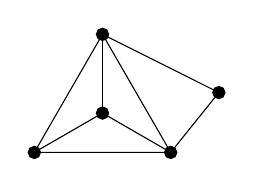
\begin{tikzpicture}
    \tikzstyle{point}=[circle,thick,draw=black,fill=black,inner sep=0pt,minimum width=4pt,minimum height=4pt]
    \node (z)[point] at (0,0) {};
    \node (a)[point] at (90:1cm) {};
    \node (b)[point] at (210:1cm) {};
    \node (c)[point] at (330:1cm) {};
    \node (d)[point] at (10:1.5cm) {};
    \path (z.center) edge (a.center);
    \path (z.center) edge (b.center);
    \path (z.center) edge (c.center);
    \draw (a.center) -- (b.center) -- (c.center) -- cycle;

    \draw (a.center) -- (d.center);
    \draw (c.center) -- (d.center);
\end{tikzpicture}
